\documentclass[12pt, a4paper, english]{report}
\usepackage[english]{babel}


\usepackage{mathtools}
\usepackage{amssymb}
\usepackage{bm}
\usepackage{upgreek}
\usepackage{amsthm}
\usepackage{xfrac}
\usepackage{thmtools}
\usepackage[binary-units=true]{siunitx}


\usepackage[T1]{fontenc}
\usepackage{mathspec}

% undo the dumb changes made by mathspec
\makeatletter
\let\RequirePackage\original@RequirePackage
\let\usepackage\RequirePackage
\makeatother

\setmonofont[
  Contextuals={Alternate}
]{Fira Code}
\usepackage{newpxtext}
\usepackage{newpxmath}
\usepackage{epsdice}
\usepackage{microtype}
\usepackage[babel]{csquotes}
\MakeOuterQuote{"}


\usepackage{tikz}
\usetikzlibrary{shapes}


\usepackage[sc,bf]{titlesec}
\newcommand{\customchapterspacing}{-1.4ex}

\titleformat
  {\chapter}
  [display]
  {\normalfont\huge\scshape\bfseries}
  {\vspace{-20pt}}
  {0pt}
  {\Huge}
  [\vspace{\customchapterspacing}\rule{\textwidth}{0.3pt}]

  \titlespacing*
{\chapter}
{0pt}
{-20pt}
{10pt}


\usepackage[toc,page]{appendix}
\usepackage{abstract}
\renewcommand{\abstractnamefont}{\normalfont\LARGE\scshape\bfseries}
\setlength{\absleftindent}{25mm}
\setlength{\absrightindent}{25mm}
\renewcommand{\abstracttextfont}{\normalfont\large}


\usepackage{graphicx}
\usepackage{subfig}
\usepackage{svg}
\graphicspath{{resources/}}

\usepackage[affil-it]{authblk}


\usepackage[
  backend=biber,
  sorting=none
]{biblatex}
\renewcommand*{\nameyeardelim}{\addcomma\space}

%% @software ~> @online
% \DeclareBibliographyAlias{software}{online}

%% decrease URL font size in bibliography
\AtBeginBibliography{\renewcommand{\UrlFont}{\ttfamily\footnotesize}}

\addbibresource{references.bib}



\usepackage[font=footnotesize,labelfont=bf]{caption}

\setlength{\abovecaptionskip}{5pt plus 1pt minus 1pt}
\setlength{\belowcaptionskip}{5pt plus 1pt minus 1pt}


\usepackage{enumitem}
\usepackage{pifont}

\newlist{todolist}{itemize}{2}
\setlist[todolist]{label=\( \square \)}
\newcommand{\cmark}{\ding{51}}
\newcommand{\xmark}{\ding{55}}
\newcommand{\done}{\rlap{\( \square \)}{\raisebox{1.5pt}{\large\hspace{1.5pt}\cmark}}\hspace{-2.5pt}}


\usepackage[margin=20mm]{geometry}
\linespread{1.15}


\usepackage{hyperref}
\usepackage{xcolor}
\hypersetup{
  colorlinks,
  linkcolor={red!50!black},
  citecolor={red!50!black},
  urlcolor={blue!50!black}
}


\usepackage{booktabs}
\usepackage{flafter}

\renewcommand{\arraystretch}{1.2}

\makeatletter
\renewcommand{\fps@figure}{htp}
\renewcommand{\fps@table}{htp}
\makeatother

\usepackage{keystroke}

\usepackage{listings}
\usepackage[minted, most]{tcolorbox}
\tcbuselibrary{minted}
\tcbuselibrary{breakable}
\usepackage{minted}

\newcommand{\customfontsize}{\fontsize{8.5}{10.2}\selectfont}

\AtBeginDocument{  % need this since listings only defines its counter after \begin{document}
\newtcblisting[auto counter, number within = chapter]{haskell}
  { listing engine=minted
  , listing only
  , minted language=haskell
  , minted options=
      { fontsize=\customfontsize
      , autogobble
      , mathescape=true
      , escapeinside=||
      }
  , before skip=10pt
  , after skip=10pt
  , breakable
  }

\newtcblisting
  [ auto counter
  , number within = chapter
  , crefname={listing}{listings}
  , Crefname={listings}{Listings}
  , blend into=listings
  ]{haskellfloat}[2]
  { listing engine=minted
  , listing only
  , blend before title=colon
  , minted language=haskell
  , minted options=
      { fontsize=\customfontsize
      , autogobble
      , mathescape=true
      }
  , before skip=10pt
  , after skip=10pt
  , breakable
  , float
  , floatplacement=htp
  , title={#1}
  , label={code:#2}
  }

\newtcblisting
  [ use counter from = haskellfloat
  , crefname={listing}{listings}
  , Crefname={listings}{Listings}
  , blend into=listings
  ]{pythonfloat}[2]
  { listing engine=minted
  , listing only
  , blend before title=colon
  , minted language=python
  , minted options=
      { linenos
      , breaklines=true
      , fontsize=\customfontsize
      , autogobble
      , mathescape=true
      , escapeinside=||
      }
  , before skip=10pt
  , after skip=10pt
  , breakable
  , float
  , floatplacement=htp
  , title={#1}
  , label={code:#2}
  }

\newtcblisting
  [ use counter from = haskellfloat
  , crefname={listing}{listings}
  , Crefname={listings}{Listings}
  , blend into=listings
  ]{myminted}[2]
  {%
  listing engine=minted,
  minted language=python,
  listing only,
  blend before title=colon,
  breakable,
  enhanced,
  minted options = {
      linenos,
      breaklines=true,
      breakbefore=.,
      fontsize=\customfontsize,
      numbersep=2mm
      , autogobble
      , mathescape=true
      , escapeinside=||
  },
  overlay={%
      \begin{tcbclipinterior}
          \fill[gray!25] (frame.south west) rectangle ([xshift=4mm]frame.north west);
      \end{tcbclipinterior}
  }
  , before skip=10pt
  , after skip=10pt
  , breakable
  , float
  , floatplacement=htp
  , title={#1}
  , label={code:#2}
}

\newtcblisting
  [ use counter from = haskellfloat
  , crefname={listing}{listings}
  , Crefname={listings}{Listings}
  , blend into=listings
  ]{cfloat}[2]
  { listing engine=minted
  , listing only
  , blend before title=colon
  , minted language=c
  , minted options=
      { fontsize=\customfontsize
      , autogobble
      , mathescape=true
      , escapeinside=||
      }
  , before skip=10pt
  , after skip=10pt
  , breakable
  , float
  , floatplacement=htp
  , title={#1}
  , label={code:#2}
  }

\newtcblisting{customtext}
  { listing engine=minted
  , listing only
  , minted language=text
  , minted options={fontsize=\customfontsize, autogobble}
  , before skip=10pt
  , after skip=10pt
  , breakable
  }
} % end \AtBeginDocument

\definecolor{hackage}{RGB}{75, 139, 190}

\newtcbox{\hackagebox}
  { enhanced
  , nobeforeafter
  , tcbox raise base
  , boxrule=0.6pt
  , top=0mm, bottom=0mm, right=0mm, left=4mm, arc=1pt
  , boxsep=1.5pt
  , before upper={\vphantom{dlg}}
  , colframe=hackage!90!black
  , coltext=hackage!25!black
  , colback=hackage!10!white
  , overlay={
      \begin{tcbclipinterior}
        \fill[hackage] (frame.south west)
        rectangle node[] {\centering
\includegraphics[width=3.5mm]{python-logo.png}}
        ([xshift=4mm]frame.north west);
      \end{tcbclipinterior}
    }
  }

\newcommand{\hackage}[1]{\hackagebox{\href{https://pypi.org/project/#1}{\color{hackage!25!black}{#1}}}}
\newcommand{\docs}[1]{\hackagebox{\href{https://docs.python.org/3/library/#1}{\color{hackage!25!black}{#1}}}}

\newcommand{\codeinlinenormal}[1]{\mintinline[fontsize=\footnotesize]{text}{#1}}
\newcommand{\codeinline}[1]{\mintinline[fontsize=\footnotesize]{text}{#1}}
\newcommand{\codeinlinesmall}[1]{\mintinline[fontsize=\scriptsize]{text}{#1}}


\makeatletter
\renewcommand\listoftables{%
  \section*{\listtablename}%
  \@mkboth{\MakeUppercase\listtablename}%
      {\MakeUppercase\listtablename}%
  \@starttoc{lot}%
}
\renewcommand\listoffigures{%
  \section*{\listfigurename}%
  \@mkboth{\MakeUppercase\listfigurename}%
      {\MakeUppercase\listfigurename}%
  \@starttoc{lof}%
}
\renewcommand\lstlistoflistings{%
  \section*{List of \lstlistlistingname}%
  \@mkboth{\MakeUppercase\lstlistlistingname}%
      {\MakeUppercase\lstlistlistingname}%
  \@starttoc{lol}%
}
\makeatother


\newcommand{\imgscaling}{0.8}
\newcommand{\customvertspacing}{0.5em}
\newcommand{\vertnegspacing}{0ex}
\newcommand{\customvertnegspacing}{0ex}
\newcommand{\aftertitlespacing}{1em}

\newcommand{\hd}{\rotatebox{60}}

\title{
  \vspace{\vertnegspacing}
  \rule{\textwidth}{1.5pt}\\[\customvertspacing]
  \huge Final Year Project Report\\[0.2em]
  \Large AI for Modified Perudo and Game Hosting Service\\[\customvertspacing]
  \rule{\textwidth}{1.5pt}\\[\aftertitlespacing]
  
\includegraphics[scale=\imgscaling]{NUIM-Crest.png}
  \vspace{\customvertnegspacing}
}

\author{
  Dheeraj Putta | 15329966\\[0.5em]
  {\small A thesis submitted in partial fulfilment of the requirements for the \\ B.Sc. Computational Thinking\\[0.5em]}
  {\small Advisor:\hspace{2mm}Dr. Phil Maguire}
}

\affil{Department of Computer Science\\Maynooth University, Ireland}

\date{March 19, 2019}


\usepackage[nameinlink]{cleveref}

\begin{document}

  \maketitle

  \begin{abstract}
    The objectives of this project were to create and implement strategies for artificial intelligence agents that could play Perudo with a modified rule set, develop code that is extensible to make it easy to add new strategies, and implement a method that allows the agents to play against each other.
    The developed agents are compared against each other but with different parameters as to compare and contrast on the effects of each of the different values. After picking the best agent from each round, the best configuration for each agent is compared against all the different agents to try and discover the best agent. Next, I compare the best agent picked against myself playing against that agent. Finally, we discuss possible improvements and other strategies that could be implemented.
  \end{abstract}

  \setcounter{tocdepth}{1}

  %% We'd like all lists to appear as sections in one big chapter.

  \tableofcontents
  \thispagestyle{empty}

  \chapter*{Lists of Floats}

  \listoftables

  \listoffigures

  \lstlistoflistings
  \thispagestyle{empty}

  \setcounter{page}{0}
  \chapter{Introduction}

Perudo is a popular dice game that is played all over the world. Perudo is a version played in South America, where it is called many different names such as Dudo, which is Spanish for \textit{I doubt}. It is more well known as Liar's Dice due to the game being called that in ``Pirates of the Caribbean'' movie franchise and the ``Red Dead Redemption'' video game series.

\section{Background}

Perudo is an example of a game with imperfect information. That is, at any point when making a decision we do not know all the information on the board. In this respect, it is similar to Poker, in Perudo we have no idea what the dice that our opponents holds are and in Poker we don't know what cards the opponent is holding. This causes difficulties in detecting possible bluffing. Hence, the optimal strategy can only be estimated with some probabilistic method that heavily depends on the opponents moves.

Perudo, however is not as difficult as Poker as it does not have as large a range of possible card combinations as well as different types of hands. From this one could think of Perudo as a simplified poker.

\section{Rules}

The majority of these games have a common rule set:
\begin{enumerate}
    \item Each player starts with 5 dice.
    \item {\large\epsdice{1}}'s are wildcards, i.e. they count as being every number.
    \item After the previous player bets that there are at least $n$ dice with a certain value, the current player has to raise the bid by raising either the number of dice, the value of the dice or both. In general you can think of each bet as having a score, defined by:
    \begin{equation}
        \label{eq:score}
        s(n, x) = 10n + x
    \end{equation}
    For example, If a player bets that there are at least 2 {\large\epsdice{3}}'s then it would have a value of 23. The current players bet is valid if the score of their bet is greater than the score of the previous bet.
    \item Only the current player may call or raise the bid.
    \item If a player calls, then all dice are revealed and the previous bet is checked. If it was a valid bet the player who has called will loose a die and a new round will start. If the bet was not valid then the previous player looses a die. Whoever looses a die will start the next round.\label{list:call}
    \item A game is finished when there is only one player left with dice.
\end{enumerate}

In Perudo there are 2 special rules that we have to consider.
\paragraph{Palafico}
When a player gets to one die, a special turn (called \textit{Palafico}) occurs. Whatever die value that player begins with cannot be changed. For example, if the \textit{Palafico} player bets that there are 2 {\large\epsdice{3}}'s, then every subsequent bet must raise that bet by saying that there are $n$ {\large\epsdice{3}}'s. A player only gets one \textit{Palafico} round per game. If they survive that round, play goes back to normal.

\paragraph{Aces}
Instead of the usual bidding, players also have the option of trying to predict how many {\large\epsdice{1}}'s there are. In this round, the number of {\large\epsdice{1}}'s predicted has to be \textbf{at least} half the previous amount. For example if the previous bet was 4 {\large\epsdice{3}} then a bet of 2 {\large\epsdice{1}} is valid. Fractions are always rounded up. After a call of \textit{Aces}, the next player may either raise the quantity of {\large\epsdice{1}}'s or they can revert back to the normal method by doubling the quantity of {\large\epsdice{1}}'s called. For example, following a bet of 3 {\large\epsdice{1}}'s, the next bid has to be at least 4 {\large\epsdice{1}}'s or 6 of any other number.

However for this project, we did not include those 2 special rules and only played with the common rule set.

\section{Example of a round}
\begin{figure}[h]
    \centering
    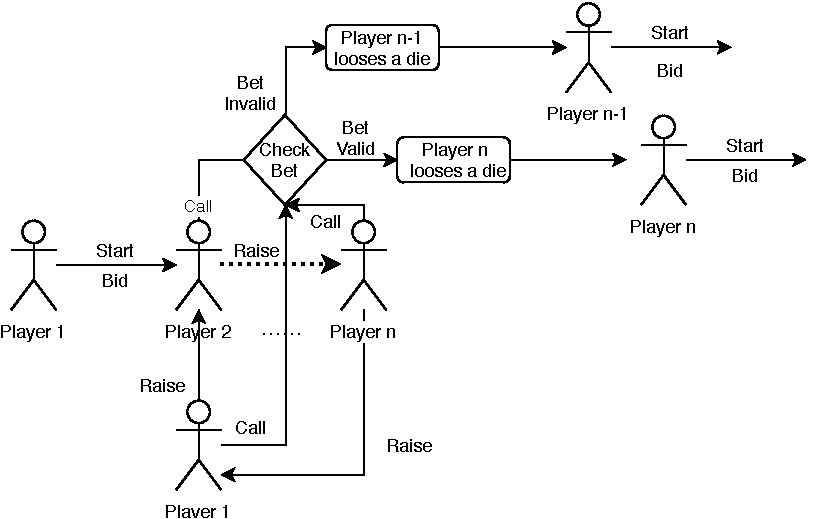
\includegraphics[width=\linewidth,page=1]{flowchart.pdf}
    \caption{Flowchart of a game of Perudo}
    \label{fig:flowcart}
\end{figure}

Using the above flowchart we will play a round of Perudo to get familiar with the rules.

Suppose that each player has the dice in \Cref{table:dicelist} and suppose that the sequence of bets seen in \Cref{fig:round} are placed.

\begin{itemize}
    \item Player 1 starts off the round with by betting 3 {\Large \epsdice{5}}'s.
    \item Player 2 then raises that bet by betting 4 {\Large \epsdice{4}}'s. This is a valid bet because if we look at \Cref{eq:score}, $s(3, 3) = 33 < s(4, 4) = 44$.
    \item Player 3 then raises this bet by betting 5 {\Large\epsdice{4}}'s. This is a valid bet because $s(5, 4) = 54 > s(4, 4) = 44$.
    \item Player 1 calls Player 3's bet. Since there were only 4 {\Large\epsdice{4}}'s, 1 {\Large\epsdice{1}} in Player 1's hand (remember that {\Large\epsdice{1}} are wild cards and count as every number) and 3 {\Large\epsdice{4}}'s in Player 2's hand, Player 3 loses a die.
    \item The round has finished and a new round starts again with Player 3 placing the starting bid.
    \item If Player 3 raised by betting 4 {\Large\epsdice{5}}'s and Player 1 called that bet, Player 1 would have lost a die as there are at least 4 {\Large\epsdice{5}}'s currently in play and a new round starts again with Player 1 starting.
\end{itemize}

\begin{table}[htbp]
    \centering
    \begin{tabular}{ccc}
        % \hline
         Player 1 &Player 2 &Player 3  \\
         \hline
         {\Large\epsdice{1}}{\Large\epsdice{3}}{\Large\epsdice{5}}{\Large\epsdice{5}}{\Large\epsdice{5}}&{\Large\epsdice{1}}{\Large\epsdice{2}}{\Large\epsdice{2}}{\Large\epsdice{4}}{\Large\epsdice{4}}& {\Large\epsdice{2}}{\Large\epsdice{3}}{\Large\epsdice{3}}{\Large\epsdice{5}}{\Large\epsdice{5}}\\
        %  \hline
    \end{tabular}
    \caption{Player's Dice}
    \label{table:dicelist}
\end{table}

\begin{figure}[htbp]
    \centering
    \begin{tikzpicture}[every node/.append style={draw, rounded corners, inner sep=5pt}]
        \node (t1) [rectangle split, rectangle split horizontal, rectangle split parts=2]
        {P1
        \nodepart{two} \Large\epsdice{5}\epsdice{5}\epsdice{5}};

        \node (t2) [rectangle split, rectangle split horizontal, rectangle split parts=2, right of=t1, xshift=2cm]
        {P2
        \nodepart{two} \Large\epsdice{4}\epsdice{4}\epsdice{4}\epsdice{4}};

        \node (t3) [rectangle split, rectangle split horizontal, rectangle split parts=2, right of=t2, xshift=2.5cm]
        {P3
        \nodepart{two} \Large\epsdice{4}\epsdice{4}\epsdice{4}\epsdice{4}\epsdice{4}};

        \node (t4) [rectangle split, rectangle split horizontal, rectangle split parts=2, right of=t3, xshift=2cm]
        {P1
        \nodepart{two} call};

        \node (t5) [rectangle split, rectangle split horizontal, rectangle split parts=2, right of=t4, xshift=2cm]
        {Verify Bet
        \nodepart{two} P3 lied};

        \draw [->, ultra thick] (t1) edge (t2) (t2) edge (t3) (t3) edge (t4) (t4) edge (t5);
    \end{tikzpicture}
    \caption{Round being played}
    \label{fig:round}
\end{figure}


\section{Approach}

Several approaches were used to try and create AI agents. First, a purely probabilistic approach was taken where the agent only considers the probability of the previous players bet when it decides whether it should raise the bet or call. Other approaches that were tried were modifications to this strategy but they took into account information such as the player's current dice and previous bets made. The final approach developed was using the MiniMax algorithm. All agents had 2 parameters that could be tweaked, one for deciding at what the cut-off probability is for deciding if a bet is false and the other parameter that decided what probability the player would bluff with.


To make the code easily extensible, an Object Oriented approach was used throughout the project.

A terminal based application was written that used TCP sockets to communicate with each player to allow them to place bets and receive updates on the game state after each player's turn. This application also allowed a number of games to be played which allows for easy simulation.

\section{Metrics}

The evaluation of the AI agents was done through 2 main methods:

\begin{itemize}
    \item \textbf{Number of wins:} This is the main metric that will be used. It allows us to measure how well the agent performs. By comparing the number of wins each of the approaches had it will allow us to evaluate how good that agent performs.
    \item \textbf{Call Accuracy:} This metric will allows us to find the approach that is the best at calling other players bluff.
\end{itemize}

Using these two metrics will help find the agent that is good at both winning and calling and not just good at one of these tasks.


  \chapter{Technical Background}

\section{Topic Material}

All of the papers mentioned in this section seem to focus on head-to-head (only 2 players) games of Perudo so they are not a direct comparison to the methods implemented in this project.


One paper \autocite{Boros2014} uses methods similar to the ones in this project except that the rule set that they used includes the \textit{Aces} rule which is not the rules used for this project. In this paper, 4 different strategies are implemented:
\begin{enumerate}
    \item A basic strategy which bids based on the basis of analysing expected values. It also takes in an extra parameter, which sets an upper bound for raising a bid. If the expected value is higher than this bound then an \textit{Aces} is called.
    \item An extended strategy -- based on the basic strategy -- which deduces back, from the initial bids, the opponent's dice. This method won more when it played against the basic strategy.
    \item A foreseeing strategy which keeps track of all bets made and tries to use that to deduce the opponents dice.
    \item A bluff strategy. This method was built from the idea that instead of winning one round it tries to win the whole game instead. This method not only considers the best theoretical build but other variations such as sending the minimum possible bet or by bluffing. The bluffing was not random and was based on the probabilities of the dice on the table, how ever no mention is made how they calculated the probabilities.
\end{enumerate}
The paper concludes that although the bluffing strategy is the best that they have implemented it still cannot be classified as a successful and "clever" player.\\

This paper \autocite{Neller2012} attempts to use a modified version of Counter Factual Minimisation (CFR) called Fixed-Strategy Iteration Counterfactual Regret Minimisation (FSICFR) to approximate an  optimal strategy for Perudo. Essentially, CFR traverses extensive game subtrees, recursing forward with reach probabilities that each player will play to each node (i.e. information set) while maintaining history, and backpropagating values and utilities used to update parent node action regrets and thus future strategy. However, due to the large size of the information set in Perudo, the number of recursive visits to nodes grew exponentially with the depth of the tree.

In FSICFR, the recursive CFR algorithm is split into two iterative passes, one forward and one backward, through a Directed Acyclic Graph (DAG). In the forward pass, visit counts and reach probabilities of each player are accumulated, yet all strategies remain fixed. (By contrast, in CFR, the strategy at a node is updated with each CFR visit.) After all the visits are counted and probabilities are accumulated, a backward pass computes utilities and updates regrets.

The new method introduced provides a quicker training time for a standard 5 die head-to-head match of Perudo compared to CFR.

\section{Technical Material}

\subsection{Socket Server}

This webpage \autocite{NathanJennings} details how to write a simple programme, using the \docs{socket} package, that accepts connections from a user, through a socket, and allows the main server to reply to these messages. It also shows examples of how to send a receive messages from multiple sources and handle them accordingly.

  \chapter{Problem Analysis}


The main goal at the start of the project was to develop and implement artificial intelligence that could play the game at a reasonable level and also to implement an extensible base to allow for the addition of new AI's. However, mid-way through the project, the goal became the development of a game hosting platform that allows humans to play against the AI as well as the AI to play against other AI.\\


One of the problems associated with developing an AI for this game is because the project requires the AI to be flexible, i.e. it must work well for any number of players. This causes a lot of the algorithms that are already used for this topic to not perform well as they are all trained on data for a head-to-head game. Another problem with trying to train models for this game is the large search space. With 4 players playing, the number of different combinations of the number of dice each player has is 625 and with 5 players it is 3125. The search space grows exponentially with the number of players in the game.\\


As well as the development of the AI, a system, as described above, had to be developed that allowed for games to be simulated between AI agents as well as gather statistics, such as win rate for each player, throughout the simulation. The system also has to allow people to use it from within the same network.



  \chapter{The Solution}

\section{Analytical Work}
\label{sec:prob}
To calculate the probability of a bet occurring, the following calculations are used.

Note that $l \in \{2, 3, 4, 5, 6\}$ and that anywhere that mentions ``occurrences of the value $l$'' should read as occurrences of the value $l$ (or {\Large\epsdice{1}}).
\begin{itemize}
    \item Since {\Large\epsdice{1}}'s are wild, this means that the probability of landing on any die face except 1 is \sfrac{1}{3}.
    \item Let $a_{n, k, l}$ be the event that among $n$ dice, there are exactly $k$ occurrences of the value $l$. Calculating the probability of $a_{n, k, l}$ amounts to rolling $k$ times the value $l$ and $ n - k$ times one of the other faces. By taking the first $k$ positions we get $2^k \times 4^{n-k}$. Now multiplying this result by the set of possible combinations of $k$ positions among $n$ dice, gives
    \[
        \binom{n}{k}2^k4^{n - k}
    \]
    We also have that $\text{Card}(\{1,2,3,4,5,6\}) = 6^n$. From this we get that
    \begin{equation}
        \label{eq:prob_a}
        P(a_{n,k,l}) = \binom{n}{k}\frac{2^k4^{n-k}}{6^n} = \binom{n}{k}\frac{2^k2^{n-k}2^{n-k}}{6^n} = \binom{n}{k}\frac{2^n2^{n-k}}{6^n} = \binom{n}{k}\frac{2^{n-k}}{3^n}
    \end{equation}

    \item Now let $A_{n, k, l}$ be the event that among $n$ dice, there are at least $k$ occurrences of the value $l$. To calculate the probability of $A_{n,k,l}$, we have to sum the probabilities for all $a_{n, i, l}$, $\forall i \in [k, n]$.
    \begin{equation}
        \label{eq:prob_a1}
        P(A_{n,k,l}) = \sum_{i = k}^n\binom{n}{i}\frac{2^{n-i}}{3^n}
    \end{equation}
    \item We can improve upon \Cref{eq:prob_a} by using the player's own dice to factor into the calculation. The event $a_{n, k ,l} \mid a_{m, j, l}$ can be interpreted as the event of having exactly $k$ occurrences of the value $l$ among $n$ dice knowing that we already have $j$ occurrences of the value $l$ among the player's $m$ dice. This is exactly the same as saying, we have exactly $k - j$ occurrences of the value $l$ among $n - m$ dice. Therefore we have
    \[
        a_{n, k ,l} \mid a_{m, j, l} = a_{n - m, k - j, l}
    \]
    and
    \begin{equation}
        \label{eq:prob_b}
        P(a_{n, k ,l} \mid a_{m, j, l}) = \binom{n - m}{k - j}\frac{2^{n-m-k+j}}{3^{n-m}}
    \end{equation}

    \item We can also improve upon \Cref{eq:prob_a1} by using the probability described in \Cref{eq:prob_b}. Let $A_{n, k ,l} \mid a_{m, j, l}$ be interpreted as having at least $k - j$ occurrences of the value $l$ among $n - m$ dice. Then
    \begin{equation}
        \label{eq:prob_b1}
        P(A_{n, k ,l} \mid a_{m, j, l}) = \sum_{i = k - j}^{n - m}\binom{n-m}{i}\frac{2^{n-m-i}}{3^{n - m}}
    \end{equation}
\end{itemize}

The implementation of \Cref{eq:prob_a1} and \Cref{eq:prob_b1} can be seen in \Cref{code:impa1} and \Cref{code:impb1}.
\section{Server Design}

The game hosting platform was built using the \docs{socket} library that comes installed with Python using the terminal as the user interface.

\subsection{Things to note}

\begin{itemize}
    \item The \docs{pickle} package is used to encode and decode data. This package implements binary protocols for serializing and de-serializing a Python object structure.\autocite{pickle}. This allows data that was encoded with \texttt{pickle} to be decoded to it's original type instead of converting the data to a string, converting that string to bytes, sending it to the player, the player converting the bytes back to a string and then to whatever type it should be. This means that the player does not need to have any idea what type the data read in should be converted to. Another advantage of using this package is that allows the server to work in both \texttt{Python2} and \texttt{Python3} as the \texttt{bytes} object that \texttt{Python3} provides does not work in \texttt{Python2}.
    \item Each player is a tuple \texttt{(conn, address)} where conn is a new socket object usable to send and receive data on the connection, and address is the address bound to the socket on the other end of the connection. So calling \texttt{player[0]}(\ref{code:p1}) allows the server to access the socket object to send information to the player.
    \item The \texttt{socket.recv()} method waits until in receives data to proceed to the next line of code.
\end{itemize}

\begin{myminted}{Sending Player information}{p1}
    player[0].sendall(pickle.dumps(self.total_dice))
    player[0].recv(131072)
    player[0].sendall(pickle.dumps(self.player_list[player].dice_list))
    player[0].recv(131072)
\end{myminted}

\subsection{Server Communication}

Using \Cref{im:inround}, the order of operations of the server will be described.

\begin{enumerate}
    \item The server sends each player the number of games they will be playing. Before sending the information to the next player, it waits until the previous player sends an ``OK'' response before continuing.
    \item Each player is sent whether the player is out and if the game is over. Similar to above the server waits until it receives a response before proceeding.
    \item If a player is not out then they are sent their dice.
    \item A player is asked to place a bet.
    \item The bet placed is then sent to all the other players.
    \item Steps 2-5 are repeated until there is only one player left with dice.
    \item After the game is finished, each player is sent a message stating if they have won or lost.
\end{enumerate}

\begin{figure}
    \centering
    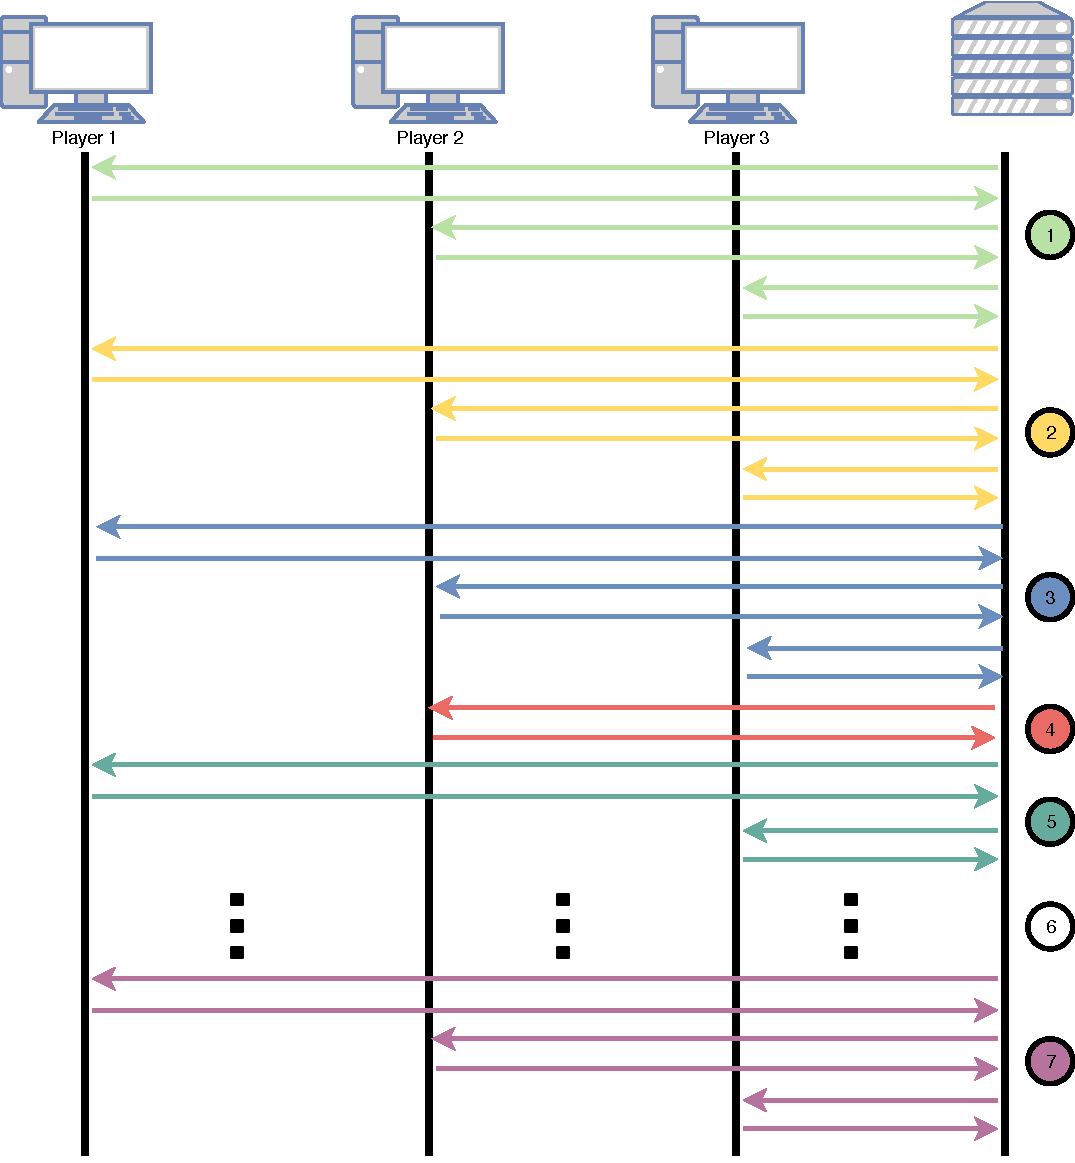
\includegraphics[width=\textwidth]{server.pdf}
    \caption{Order of operation during a game}
    \label{im:inround}
\end{figure}

\section{Methods}
\label{sec:methods}
\subsection{Generating Bets}

The amount of dice to bet on were generated randomly using a skewed normal distribution using the \hackage{scipy} package and the die value to bet on was generated using previous bets. The implementation can be seen in \Cref{code:genbets}.

\noindent The skewed PDF implementation in \texttt{scipy} is generated using

\begin{align*}
    PDF_{\text{Skew}}(x, a, l, s) &= \frac{2 * PDF(y) * CDF(a * y)}{s} \\
    y &= \frac{x - l}{s}
\end{align*}

where $a$ is a skewness parameter, $l$ is a location parameter, $s$ is a scaling parameter and $PDF$ and $CDF$ are the probability density function and cumulative density function, respectively, of the normal distribution. The graph seen in \Cref{im:skewnorm} was generated with $a = 5, l = .5, s = 4$.

\begin{figure}
\centering
\subfloat[PDF of a Skewed Normal Distribution]{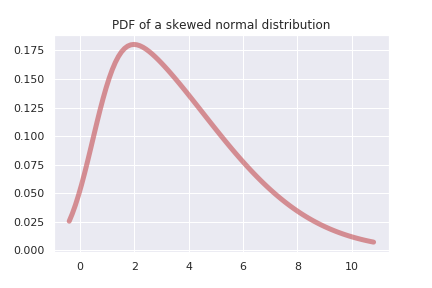
\includegraphics[width=.45\textwidth]{skewnorm.png}\label{im:skewnorm}}
\hfill
\subfloat[Probability of a bet with 10 dice in play]{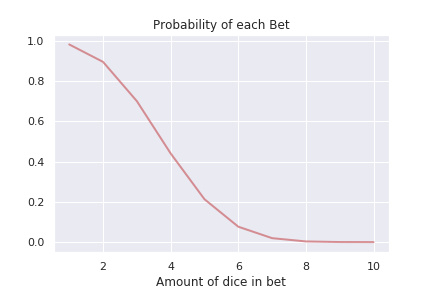
\includegraphics[width=.45\textwidth]{diceprob.png}\label{im:diceprob}}
\caption{Skewnorm compared to dice probability}
\end{figure}

A skewed distribution was used as, when placing bets, it is usually safer to place a low number of a die value. If a standard normal distribution was used instead of a skewed distribution, every amount would be just a likely when generating bets. However in the game this is not the case as bets that contain a high dice number a less likely to occur as seen in \Cref{im:diceprob}, where the $x$-axis is the amount of dice that you are betting are on the table.\\

The die value itself was generated using bets made throughout the round. The code is more likely to generate a number that has already been bet on as it is more likely that there are more dice on the table, with a die value that has already been bet on.

\subsection{Improving the Probability Formula}

The formulas seen in \Cref{sec:prob} do not take into account the bets that have been made in the current round. Suppose that $D$ is a dictionary containing the numbers 2 to 6 as the keys and the values being the highest amount of that die value that has been bet. Then
\begin{equation}\label{eq:fkl}
    f(k, l) = P(A_{n, k, l} | a_{m, j, l}) + D[l]
\end{equation}
where $j, k, l, m$ and $n$ are as described in \Cref{eq:prob_b1}. Note that this is no longer a probability but rather a score metric as we can obtain values larger than 1. The implementation can be seen in \Cref{code:fkl}

\subsection{Minimax}

Minimax is a depth-first depth-limited search which examines all states . There are 2 phases in the algorithm
\begin{enumerate}
    \item Descend the search tree up to the depth limit and apply the heuristic function.
    \item Propagate those values up the tree.
\end{enumerate}

The basic idea of Minimax is that during your move you want to maximize the heuristic value, as this is the best move for you, while the opponent tries to minimize the heuristic value as this will result in you performing a worse move.

\subsubsection{Example of Minimax}
\begin{figure}
    \centering
    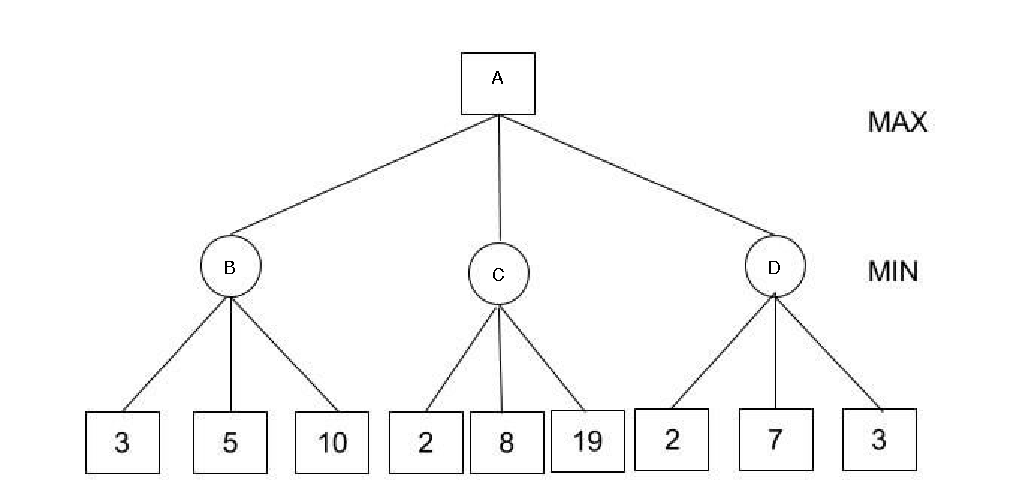
\includegraphics[width=\textwidth]{minimax.pdf}
    \caption{Minimax Tree}
    \label{im:minimax}
\end{figure}

We traverse the tree depth-first, starting from the left branch.

\begin{enumerate}
    \item Since B is a minimizer, it will pick the child node that has the lowest heuristic value. In this case B now has a value of 3.
    \item C is a minimize so it will pick the node that has a heuristic value of 2. Now C has a heuristic value for 2.
    \item D is a minimize, so it picks the child with a heuristic value of 2. D now has a value of 2.
    \item Since A is a maximizer, it picks the child node with the highest heuristic value. In this case that would B.
    \item Therefore we will perform the action that node B represents.
\end{enumerate}

The implementation for this can be seen in \Cref{code:minimaximp}

\subsection{$\alpha$--$\beta$ pruning}

The problem with regular Minimax is that it is an exhaustive method that explores unnecessary search spaces causing the algorithm to be slow and inefficient. For this reason $\alpha$--$\beta$ pruning will be used.

In $\alpha$--$\beta$ pruning there are two threshold values:
\begin{itemize}
    \item $\alpha$, which represents the lower bound of a maximizing level.
    \item $\beta$, which represents the upper bound of the minimizing level.
\end{itemize}

We terminate a search when we are
\begin{itemize}
    \item below a max node with $\alpha \geq \beta$ of any of it's min ancestors.
    \item below a min node with $\alpha \geq \beta$ of any of it's max ancestors.
\end{itemize}

Let $b$ be the number of children for each node and $m$ is the maximum depth of the tree then:
\begin{itemize}
    \item For regular MiniMax, the time complexity is $\mathcal{O}(b^m)$.
    \item For MiniMax with $\alpha$--$\beta$ pruning, the time complexity is $\mathcal{O}(b^{m/2})$
\end{itemize}

With the termination rules above, we can easily modify the implementation seen in \Cref{code:minimaximp} so that it implements $\alpha$--$\beta$ pruning, as seen in \Cref{code:abpruning}

\subsubsection{Example}

We will work through a partial example of how $\alpha$--$\beta$ pruning works by looking at the tree below.

\begin{figure}
    \centering
    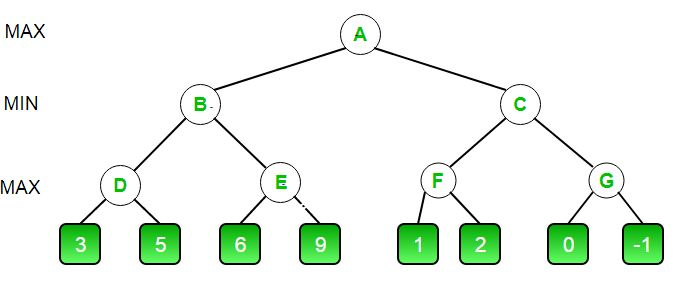
\includegraphics[width=\textwidth]{MIN_MAX1.jpg}
\end{figure}

\begin{enumerate}
    \item The initial call starts from A. Initially, $\alpha = -\infty$ and $\beta=\infty$. These values are passed down to subsequent nodes in the tree. We then explore the left branch of the tree.
    \item At D, it has $\alpha = -\infty$ and $\beta = \infty$ as these are inherited from A.
    \item D looks at it's left child which returns a value of 3. Now $\alpha = \max(-\infty, 3) = 3$.
    \item Since $\alpha = 3 \not\geq \beta$ we continue searches other children of D.
    \item D looks at it's right child which returns a value of 5. Now $\alpha = \max(3, 5) = 5$.
    \item D then returns a value of 5 to $B$. Now B has $\beta = \min(\infty, 5) = 5$.
    \item Now the right child of B is explored. At E, $\alpha = -\infty$ and $\beta = 5$.$\beta \neq \infty$ as B passes it's value down to E.
    \item E looks at it's left child, which returns 6. Now $\alpha = \max(-\infty, 6) = 6$.
    \item Since $\alpha = 6 \geq \beta = 5$, we do not need to check the other child of E. This is because B is a minimizing node and as D guarantees that it will return \underline{at most} 5, while after exploring the left child of E, we know it will return \underline{at least} 6, Therefore exploring along the right child of E is useless as we will never pick E.
\end{enumerate}

After performing the algorithm on the whole tree, we end up with the resulting search space seen in \Cref{im:finaltree}

\begin{figure}
    \centering
    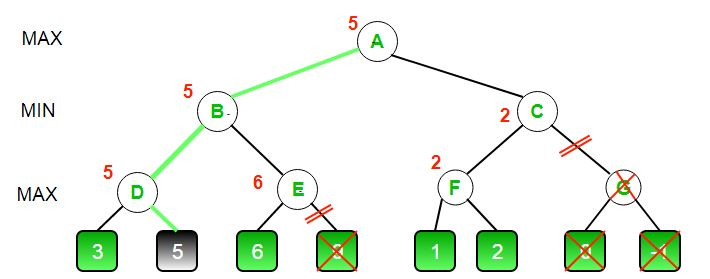
\includegraphics[width=\textwidth]{MIN_MAX3.jpg}
    \caption{Final Tree after performing $\alpha$--$\beta$ pruning}
    \label{im:finaltree}
\end{figure}

In this example we saved time compared to the regular Minimax algorithm by not exploring 3 nodes. In larger graphs the number of nodes that are not explored in the $\alpha$--$\beta$ pruning version of Minimax is a lot larger than this. This means we save time searching and this allows us to search more nodes in the same amount of time.



\section{Class Structure}

\begin{figure}
    \centering
    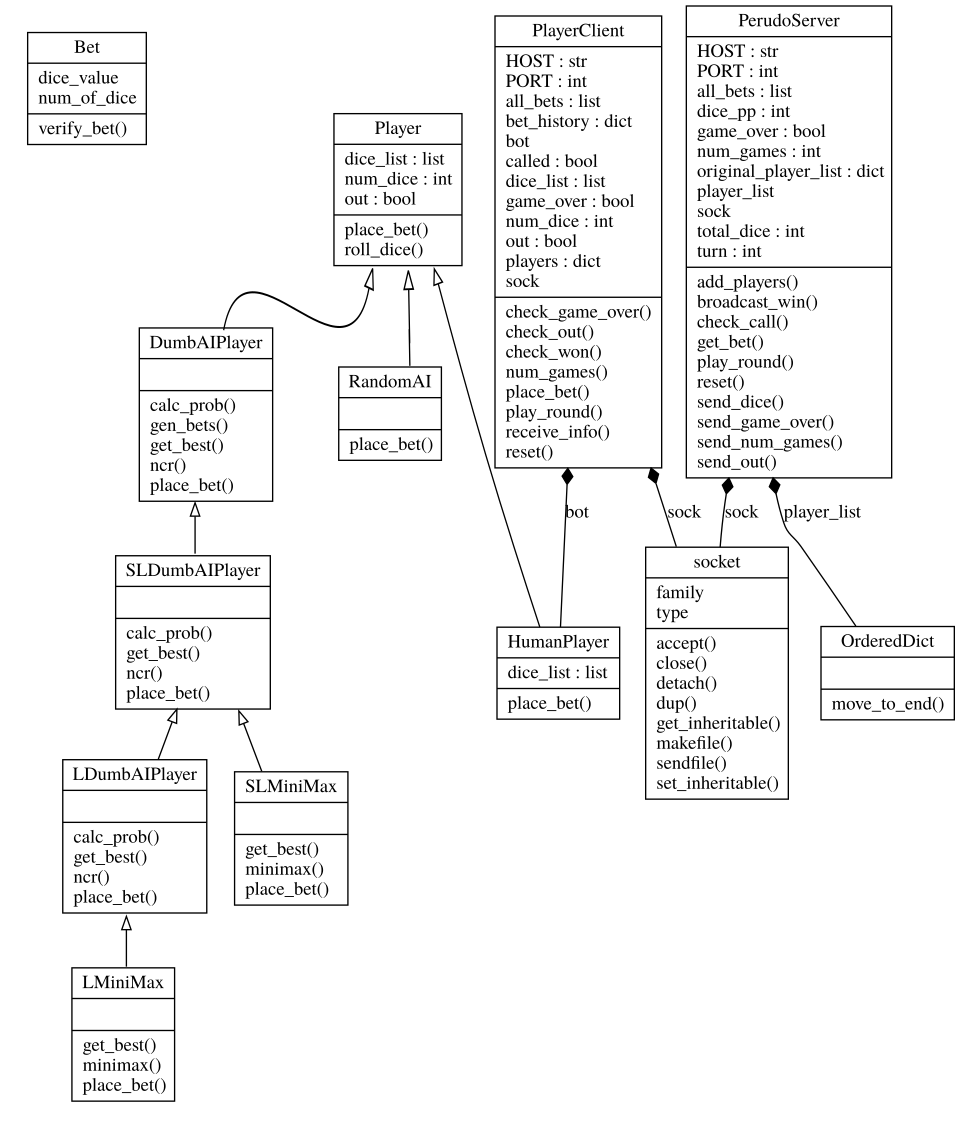
\includegraphics[width=\textwidth]{classes.png}
    \caption{UML Class Diagram of Project}
    \label{fig:class}
\end{figure}

The class structure of the project this project can see seen in \Cref{fig:class} and the dependency graph can be seen in \Cref{fig:package}.

\begin{figure}
    \centering
    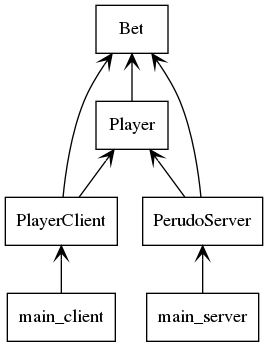
\includegraphics[scale=.5]{packages.png}
    \caption{Package Structure of Project}
    \label{fig:package}
\end{figure}

\section{Implementation}
\subsection{Strategy for AIPlayer's}

The general strategy for all the AI's except MiniMax is as follows
\begin{enumerate}
    \item If you are placing a starting bet then bet that there are at least 2 to 4 dice of some number.
    \item If you are not placing a starting bet, then generate bets using the method seen in \Cref{sec:methods}.
    \item If the probability (or score), calculated using \Cref{eq:prob_a1} for \texttt{DumbAIPlayer} and \Cref{eq:prob_b1} for \texttt{SLDumbAIPlayer} and \Cref{eq:fkl} for \texttt{LDumbAIPlayer}, for any bet is less than the \texttt{prob} value passed into the function then the AI calls the previous players bet and goes back to step 1.
    \item Otherwise, the AI then places a random bet from the generated bets with a probability given by the \texttt{bluff} variable or it places the bet from the generate bets that has the highest probability.
\end{enumerate}
The actual implementation for placing bets can be seen in \Cref{code:getbest}.

\subsection{Strategy for MiniMax}

The strategy that the both \texttt{LMiniMax} and \texttt{SLMiniMax} players is as follows
\begin{enumerate}
    \item If you are placing a starting bet then bet that there are at least 2 to 4 dice of some number.
    \item If you are not placing a starting bet, then run the \texttt{minimax()} method (\Cref{code:abpruning})
    \item If the score, calculated using \Cref{eq:fkl} for \texttt{LMiniMax} and \Cref{eq:prob_b1} for \texttt{SLMiniMax}, for the bet returned by the \texttt{minimax()} method is less than the \texttt{prob} value passed into the function then the AI calls the previous players bet and goes back to step 1.
    \item Otherwise, either the AI places a random bet like above or it places the bet output by the \texttt{minimax()} method.
\end{enumerate}
The implementation can be seen in \Cref{code:mmbet}.

  \chapter{Evaluation}

The success of the AI's was measured by using the accuracy of the calls it made and the number of games it won as well. During the testing the order of the players was shuffled to ensure that the same players do not follow after each other and to prevent the same player going last in a round as whoever went last did better as they had the most information.

\section{Selecting Parameters}
All the AI's had to be tested against themselves but with different parameters to try and obtain the ideal values for \texttt{bluff} and \texttt{prob} for each AI. This test was done using 100 games.

\begin{table}
    \centering
    \begin{tabular}{l|ccc}
        &.1&.25&.4\\
        \hline
        .1&92.72\%, 7& 83.75\%, 5& 83.33\%, 0\\
        .25&74.2\%, 23& 73.29\%, 18& 75.41\%, 4\\
        .4&69.27\%, 18& 69.11\%, 13& 69.06\%, 12
    \end{tabular}
    \caption{\texttt{prob} v.s. \texttt{bluff} for \texttt{DumbAIPlayer}}
    \label{table:res1}
\end{table}

As we can see \texttt{DumbAIPlayer} works the best with \texttt{prob} = .25 and \texttt{bluff} = .25.

\begin{table}
    \centering
    \begin{tabular}{l|ccc}
        & .1& .25& .4\\
        \hline
        .1&86.9\%, 10& 77.65\%, 11& 84.36\%, 2\\
        .25&76.52\%, 24& 76.64\%, 18& 70.85\%, 4\\
        .4&65.1\%, 12& 68.81\%, 16& 64.76\%, 3
    \end{tabular}
    \caption{\texttt{prob} v.s. \texttt{bluff} for \texttt{SLDumbAIPlayer}}
    \label{table:res2}
\end{table}

As we can see \texttt{SLDumbAIPlayer} works the best with \texttt{prob} = .25 and \texttt{bluff} = .1. These are also the values that are used for \texttt{SLMiniMax}.

\begin{table}
    \centering
    \begin{tabular}{l|ccc}
        &.1&.25&.4\\
        \hline
        .1&25.02\%, 12& 18.45\%, 5& 15.08\%, 2\\
        .25&64.6\%, 16& 62.43\%, 14& 56.78\%, 10\\
        .4&66.46\%, 22& 66.32\%, 9& 65.34\%, 10
    \end{tabular}
    \caption{\texttt{prob} v.s. \texttt{bluff} for \texttt{LDumbAIPlayer}}
    \label{table:res3}
\end{table}

As we can see \texttt{LDumbAIPlayer} works the best with \texttt{prob} = .4 and \texttt{bluff} = .1. These are also the values that are used for \texttt{LMiniMax}.

\section{Results and Analysis}


\subsection{Results}

500 games were simulated to obtain the results seen in the table below.

\begin{table}
    \centering
    \begin{tabular}{l|l|l}
        Type of AI&Call Accuracy & Games Won\\
        \hline
        \texttt{DumbAIPlayer} & 64.71\% & 65\\
        \texttt{SLDumbAIPlayer} & 75.95\% & 200\\
        \texttt{LDumbAIPlayer} & 68.91\% & 225\\
        \texttt{SLMiniMax} & 40.4\% & 0\\
        \texttt{LMiniMax} & 43.16\% & 0\\
        \texttt{RandomAI} & 9\% & 0
    \end{tabular}
    \caption{Call Accuracy and Number of games won for each AI}
    \label{table:res6}
\end{table}

After this, a human played against \texttt{LDumbAIPlayer} and the results are collected below.

\begin{table}
    \centering
    \begin{tabular}{l|l|l|l}
        Player & Call Accuracy & Games Won & Average Number of Dice\\
        \hline
        Human & 35.75\% & 9& 2.6\\
        \texttt{LDumbAIPlayer} & 35\% & 11 & 3.2
    \end{tabular}
    \caption{Call Accuracy, Number of Games won and the Average number of dice left when won}
    \label{table:res7}
\end{table}
\subsection{Analysis of Results}

From \Cref{table:res6}, we can gather the following:
\begin{enumerate}
    \item All of the AI's are better than the baseline \texttt{RandomAI} bot.
    \item \texttt{LDumbAIPlayer} is the best AI developed as it has won the most games, however it is not as good as \texttt{SLDumbPlayer} at correctly calling. Perhaps this could be fixed by further tweaking the value of \texttt{prob} for \texttt{LDumbAIPlayer}.
    \item The fact that both \texttt{SLMiniMax} and \texttt{LMiniMax} win no games is very surprising. Perhaps the extra information received by using a Minimax tree is detrimental to the way the game is treated in this project.
\end{enumerate}

From \Cref{table:res7}, we can see that \texttt{LDumbAIPlayer} is about as good as the human playing against it.

  \chapter{Conclusions}

\section{Project Approach}

The approach for this project was to try and develop a code base that be easily built on and improved. To implement any other AI, one would have to have a class that inherits from the \texttt{Player} class and implements the \texttt{place\_bet()} method and uses the \texttt{check\_bet()} method to check if their bet is valid. After that you would have to add it to the \texttt{players} dictionary in the \texttt{PlayerClient.py} file.

\section{Results Discussion}

The results achieved by the algorithms developed in this project are good however due to the the way the parameters were selected it may not be as good as it could be. Playing each AI against a version of itself but with different parameters may not be a good idea as they all follow the same strategy. Maybe a better idea would be to try and play a number of games with every AI but with different parameters however this would involve playing 100 games with 27 players, which would take a long time. Also running the AI for more than 100 games each would provide more reliable results for the parameters.

Another problem with my approach is that I use the values of .1, .25 and .4 for the parameters but there may be better values which are being ignored.

\section{Future Work}

\begin{itemize}
    \item To further improve upon this project one could develop a web interface. This would allow for an easier experience of playing the game against the AI as one would not need to have the Python files locally. This would also help with testing the quality of each of the AI's as it would allow for more wide spread play.
    \item The AI's seem to call unnecessarily more often when they get to a low amount of dice. With this problem addressed, I believe that the AI would perform even better.
    \item Something else that could be done to improve the project would be to allow for a player to keep track of all the other players bets and the amount of dice they have. Currently, only the dice the player has themselves is stored however with this improvement I believe this would allow more strategies based on probability to be implemented.
    \item Another AI could be implemented that instead of using just what \texttt{LDumbAIPlayer} used, it would also use the number of times that a bet with a certain die value has been place rather than just the largest bet on that die value.
    \item Given more time, it would be possible to use using strategies such as Reinforcement Learning or Neural Networks to create AI that models the game in a way that is not purely probabilistic. However the problem of having the model created be able to play with any numbers players still exists.
\end{itemize}


  \clearpage % or \cleardoublepage
  \addcontentsline{toc}{chapter}{Bibliography}
  \nocite{*}
  \printbibliography

  \begin{appendices}
    \chapter{Appendix A}
    \label{ch:apA}

    \begin{myminted}{Generating Bets}{genbets}
        def gen_bets(self, total_dice, bet_history, last_bet=None, num_bets=50):
            if last_bet:
                bets = set()
                i = 0
                probs = skewnorm.pdf(range(last_bet.num_of_dice, total_dice + 1), 5, .5, 4)
                probs = probs / sum(probs)
                dice_probs = [1/5 for _ in range(5)]
                for die in bet_history.keys():
                    dice_probs[i - 2] += bet_history[die] / 100
                dice_probs = [x/sum(dice_probs) for x in dice_probs]
                while len(bets) != num_bets and i < 150:
                    die_value = int(choice(range(2, 7), 1, p=dice_probs)[0])
                    die_amount = int(choice(range(last_bet.num_of_dice, total_dice + 1), 1, p=probs)[0])
                    bet = Bet(die_value, die_amount)
                    if bet.verify_bet(total_dice, last_bet, verbose=False):
                        bets.add(bet)

                    i += 1

                return list(bets)

            return [Bet(x, y) for x in range(2, 7) for y in range(1, 4)]
    \end{myminted}

    \chapter{Appendix B}

    \begin{myminted}{\Cref*{eq:prob_a1}}{impa1}
        def calc_prob(self, total_dice, dice_value, num_of_dice):
            return sum([self.ncr(total_dice, i) * (2**(total_dice - i) / 3**total_dice)
                        for i in range(num_of_dice, total_dice + 1)])
    \end{myminted}

    \begin{myminted}{\Cref*{eq:prob_b1}}{impb1}
        def calc_prob(self, total_dice, dice_value, num_of_dice):
            end_index = total_dice - len(self.dice_list)
            our_dice = self.dice_list.count(dice_value) + self.dice_list.count(1)
            start_index = num_of_dice - our_dice
            return sum([self.ncr(end_index, i) * (2**(end_index - i)) / (3**end_index)
                        for i in range(start_index, end_index + 1)])
    \end{myminted}

    \begin{myminted}{\Cref*{eq:fkl}}{fkl}
        def calc_prob(self, total_dice, dice_value, num_of_dice, bet_history):
            end_index = total_dice - len(self.dice_list)
            our_dice = self.dice_list.count(dice_value) + self.dice_list.count(1)
            start_index = num_of_dice - our_dice
            prob = sum([self.ncr(end_index, i) * 2**(end_index - i) / 3**end_index
                        for i in range(start_index, end_index + 1)])
            prob += bet_history[dice_value] / 100
            return prob
    \end{myminted}

    \begin{myminted}{Placing a bet}{getbest}
        def get_best(self, total_dice, bet_history, prob, bluff, last_bet):
            if not last_bet and len(self.dice_list) == 1:
                return Bet(self.dice_list[0], 1)
            elif len(self.dice_list) == 1:
                return "call"
            else:
                bets = super().gen_bets(total_dice, last_bet)
                probs = [self.calc_prob(total_dice, bet.dice_value, bet.num_of_dice, bet_history, last_bet) for bet in bets]
                index, value = max(enumerate(probs), key=op.itemgetter(1))
                # print(probs)
                if value <= prob:
                    return "call"
                else:
                    if randint(1, int(1/bluff)) == 1:
                        return bets[randint(0, len(bets) - 1)]

                    return bets[index]
    \end{myminted}

    \chapter{Appendix C}

    \begin{myminted}{Minimax Implementation}{minimaximp}
        def minimax(self, total_dice, last_bet, max_turn=True, max_depth=4):
            if max_depth == 0:
                return (last_bet, super().calc_prob(total_dice, last_bet.dice_value, last_bet.num_of_dice) * (1 if not max_turn else -1))

            bets = super().gen_bets(total_dice, last_bet, 10)

            best_value = float('-inf') if max_turn else float('inf')
            bet_to_make = ""

            for bet in bets:
                bet_to_place, value = self.minimax(total_dice, bet, not max_turn, max_depth - 1)

                if value > best_value and max_turn:
                    best_value = value
                    bet_to_make = bet

                if value < best_value and not max_turn:
                    best_value = value
                    bet_to_make = bet
            return (bet_to_make, best_value)
    \end{myminted}

    \begin{myminted}{Minimax with $\alpha$ - $\beta$ pruning}{abpruning}
        def minimax(self, alpha, beta, total_dice, last_bet, max_turn=True, max_depth=4):
            if max_depth == 0:
                return (last_bet, super().calc_prob(total_dice, last_bet.dice_value, last_bet.num_of_dice) * (1 if not max_turn else -1))

            bets = super().gen_bets(total_dice, last_bet, 10)

            best_value = float('-inf') if max_turn else float('inf')
            bet_to_make = ""

            for bet in bets:
                bet_to_place, value = self.minimax(alpha, beta, total_dice, bet, not max_turn, max_depth - 1)

                if value > best_value and max_turn:
                    best_value = value
                    bet_to_make = bet
                    alpha = max(alpha, best_value)
                    if beta <= alpha:
                        break

                if value < best_value and not max_turn:
                    best_value = value
                    bet_to_make = bet
                    beta = min(beta, best_value)
                    if beta <= alpha:
                        break
            return (bet_to_make, best_value)
    \end{myminted}

    \begin{myminted}{Placing a Bet with MiniMax}{mmbet}
        def get_best(self, total_dice, bet_history, prob, bluff, last_bet):
            if not last_bet and len(self.dice_list) == 1:
                return Bet(self.dice_list[0], 1)
            elif len(self.dice_list) == 1:
                return "call"
            else:
                bet, _ = self.minimax(float('-inf'), float('inf'), total_dice, bet_history, last_bet)
                bet_prob = super().calc_prob(total_dice, bet.dice_value, bet.num_of_dice, bet_history)
                # print("Final bet was: {} with probability {}".format(repr(bet), bet_prob))
                if bet_prob < prob:
                    return 'call'
                elif randint(1, int(1/bluff)) == 1:
                    bets = super().gen_bets(total_dice, bet_history, last_bet)
                    probs = [self.calc_prob(total_dice, bet.dice_value, bet.num_of_dice, bet_history) for bet in bets]
                    if not probs:
                        return "call"

                    sorted_bets = [(x, y) for x, y in sorted(list(zip(probs, bets)), key=lambda pair: -pair[0])]

                    return sorted_bets[randint(0, int(len(sorted_bets) / 2))][1]

                return bet
    \end{myminted}
\end{appendices}


\end{document}
